%%%%%%%%%%%%%%%%%%%%%%%%%%%%%%%%%%%%%%%%%%%%%%%%%%%%%%%%%%%%
\documentclass[a4paper,11pt,oneside]{article}
\usepackage[a4paper,vmargin={1.5cm,1.5cm},width=17cm]{geometry}
\usepackage[style=verbose-inote,doi=false,sortcites=true,block=space,backend=bibtex]{biblatex}
\usepackage[utf8]{inputenc}
\usepackage{textcomp}
\usepackage[english]{babel}
\usepackage{microtype}
\usepackage{lmodern}
\usepackage{graphicx}
\usepackage{fancyhdr}
\usepackage{booktabs}
\usepackage{eurosym}
\usepackage{hyperref}

%%%%%%%%%%%%%%%%%%%%%%%%%%%%%%%%%%%%%%%%%%%%%%%%%%%%%%%%%%%%
%% HEADERS
\setlength{\headheight}{1cm}
\setlength{\headsep}{0.5cm}
\pagestyle{fancyplain}
\fancyhf{}
\lhead{\fancyplain{}{\sc Grant Proposal }}
\rhead{\fancyplain{}{\sc NEXT}}
\cfoot{\thepage}
\renewcommand{\headrulewidth}{0pt} % remove lines
\renewcommand{\footrulewidth}{0pt}

%%%%%%%%%%%%%%%%%%%%%%%%%%%%%%%%%%%%%%%%%%%%%%%%%%%%%%%%%%%%
%% Hack to make math formulas bold in section titles
\makeatletter
\DeclareRobustCommand*{\bfseries}{%
  \not@math@alphabet\bfseries\mathbf
  \fontseries\bfdefault\selectfont
  \boldmath
}
\makeatother

%%%%%%%%%%%%%%%%%%%%%%%%%%%%%%%%%%%%%%%%%%%%%%%%%%%%%%%%%%%%
\def\thesection{\bf \textsf{\alph{section}}}

%\nobibliography{biblio}
%\bibliographystyle{JHEP}

\bibliography{biblio}


%%%%%%%%%%%%%%%%%%%%%%%%%%%%%%%%%%%%%%%%%%%%%%%%%%%%%%%%%%%%
\begin{document}

%% Some useful definitions
% BB
\newcommand{\bb}{\ensuremath{\beta\beta}}
% BB0NU
\newcommand{\bbonu}{\ensuremath{\beta\beta0\nu}}
% BB2NU
\newcommand{\bbtnu}{\ensuremath{\beta\beta2\nu}}
% NME
\newcommand{\Monu}{\ensuremath{\Big|M_{0\nu}\Big|}}
\newcommand{\Mtnu}{\ensuremath{\Big|M_{2\nu}\Big|}}
% PHASE-SPACE FACTOR
\newcommand{\Gonu}{\ensuremath{G_{0\nu}(\Qbb, Z)}}
\newcommand{\Gtnu}{\ensuremath{G_{2\nu}(\Qbb, Z)}}

% mbb
\newcommand{\mbb}{\ensuremath{m_{\beta\beta}}}
\newcommand{\kgy}{\ensuremath{\rm kg \cdot y}}
\newcommand{\ckky}{\ensuremath{\rm counts/(keV \cdot kg \cdot y)}}
\newcommand{\mbba}{\ensuremath{m_{\beta\beta}^a}}
\newcommand{\mbbb}{\ensuremath{m_{\beta\beta}^b}}
\newcommand{\mbbt}{\ensuremath{m_{\beta\beta}^t}}
\newcommand{\nbb}{\ensuremath{N_{\beta\beta^{0\nu}}}}

% Qbb
\newcommand{\Qbb}{\ensuremath{Q_{\beta\beta}}}

% Tonu
\newcommand{\Tonu}{\ensuremath{T_{1/2}^{0\nu}}}

% Tonu
\newcommand{\Ttnu}{\ensuremath{T_{1/2}^{2\nu}}}

% Xe-136
\newcommand{\Xe}{\ensuremath{^{136}}Xe}

% Xe-136
\newcommand{\CS}{\ensuremath{^{137}}Cs}

% Xe-136
\newcommand{\NA}{\ensuremath{^{22}}Na}


% Bi-214
\newcommand{\Bi}{\ensuremath{^{214}}Bi}

% Tl-208
\newcommand{\Tl}{\ensuremath{^{208}}Tl}

% Pb-208
\newcommand{\Pb}{\ensuremath{^{208}}Pb}
% Pb-208
\newcommand{\PBD}{\ensuremath{^{210}}Pb}

% Po-214
\newcommand{\Po}{\ensuremath{^{214}}Po}

% bru
\newcommand{\bru}{cts/(keV$\cdot$kg$\cdot$y)}

% Saltos de carro en tablas
\newcommand{\minitab}[2][l]{\begin{tabular}{#1}#2\end{tabular}}

\newcommand{\thedraft}{0.1.1}% version for referees

\newcommand{\MO}{\ensuremath{{}^{100}{\rm Mo}}}
\newcommand{\SE}{\ensuremath{{}^{82}{\rm Se}}}
\newcommand{\ZR}{\ensuremath{{}^{96}{\rm Zr}}}
\newcommand{\KR}{\ensuremath{{}^{82}{\rm Kr}}}
\newcommand{\ND}{\ensuremath{{}^{150}{\rm Nd}}}
\newcommand{\XE}{\ensuremath{{}^{136}\rm Xe}}
\newcommand{\GE}{\ensuremath{{}^{76}\rm Ge}}
\newcommand{\GES}{\ensuremath{{}^{68}\rm Ge}}
\newcommand{\TE}{\ensuremath{{}^{128}\rm Te}}
\newcommand{\TEX}{\ensuremath{{}^{130}\rm Te}}
\newcommand{\TL}{\ensuremath{{}^{208}\rm{Tl}}}
\newcommand{\CA}{\ensuremath{{}^{48}\rm Ca}}
\newcommand{\CO}{\ensuremath{{}^{60}\rm Co}}
\newcommand{\PO}{\ensuremath{{}^{214\rm Po}}}
\newcommand{\U}{\ensuremath{{}^{235}\rm U}}
\newcommand{\CT}{\ensuremath{{}^{10}\rm C}}
\newcommand{\BE}{\ensuremath{{}^{11}\rm Be}}
\newcommand{\BO}{\ensuremath{{}^{8}\rm Be}}
\newcommand{\UDTO}{\ensuremath{{}^{238}\rm U}}
\newcommand{\CD}{\ensuremath{^{116}{\rm Cd}}}
\newcommand{\THO}{\ensuremath{{}^{232}{\rm Th}}}
\newcommand{\BI}{\ensuremath{{}^{214}}Bi}


%% Heading
\begin{center}
{\Large \textsf{Convocatorias 2014}} \\ \vspace{0.3cm}
{\Large  \textsf{Proyectos de I+D ``Excelencia'' y Proyectos de I+D+I ``Retos Investigación"}} \\ 
{\Large \textsf{Dirección General de Investigación Científica y Técnica}} \\
{\Large \textsf{Subdirección General de Proyectos de Investigación }} \\ 
%\vspace{0.5cm}
%{\LARGE \bf \textsf{Construcción puesta a punto y operación del experimento NEXT en el Laboratorio Subterráneo de Canfranc} }\\ 
%\vspace{0.3cm}
%{\LARGE \bf \textsf{Construction, commissioning and operation of the NEXT experiment at the Canfranc Underground Laboratory }}\\ 
\end{center}


\section{\bf \textsf{SUMMARY OF THE PROPOSAL}}

{\sc Coordinator:} Juan José Gómez Cadenas.
\vspace{0.3cm}

{\sc Title of project:} Construction, commissioning, operation and R\&D for the NEXT experiment at the LSC.
\vspace{0.3cm}

{\sc ACRONYM OF THE COORDINATED PROJECT:} NEXT.
\vspace{0.3cm}

{\sc Groups participating in project:} Instituto de Física Corpuscular (IFIC), Universidad Politécnica de Valencia (UPV), Universidad de Santiago (US) \& Centro de Láseres Pulsados (CLPU). 
\vspace{0.3cm}

{\bf SUMMARY OF THE COORDINATED PROJECT:} 
\vspace{0.3cm}

%%

NEXT (Neutrino Experiment with a Xenon TPC) is an experiment to search neutrino less double beta decay processes (\bbonu). The detection of such processes would demonstrate that neutrinos are Majorana particles (that is their own antiparticles) and would have deep consequences in physics and cosmology.  

The isotope chosen by NEXT is  \XE. The collaboration has access to hundred kilograms of xenon enriched at 90\% in \XE, owned by the Underground Laboratory of Canfranc (LSC). The NEXT technology is based in the use of time projection chambers operating at a typical pressure of 15 bar and using electroluminescence to amplify the signal (\HPXE). The main advantages of the experimental technique are: a) excellent energy resolution; b) the ability to reconstruct the trajectory of the two electrons emitted in the decays, a unique feature of the \HPXE\ which further contributes to the suppression of backgrounds; c) scalability to large masses; and d) the possibility to reduce the background to negligible levels thanks to the barium tagging technology (\BATA).

The NEXT roadmap was designed in four stages: i) Demonstration of the \HPXE\ technology with prototypes deploying a mass of natural xenon in the range of 1 kg; ii) Characterisation of the backgrounds to the \bbonu\ signal and measurement of the \bbtnu\ signal with the NEW detector, deploying 12 kg of enriched xenon and operating at the LSC; iii) Search for \bbonu\ decays with the NEXT-100 detector, which escales up the NEW detector by a factor 2:1 in size (8:1 in mass) and deploys, thus, 100 kg of enriched xenon. iv) Search for \bbonu\ decays with the BEXT detector (Barium-tagging Experiment with a Xenon TPC), which will deploy a mass in the ton scale and will introduce the technology of \BATA\ in order to reduce backgrounds to negligible levels.  

The first stage of NEXT has been successfully completed during the period 2009-2013. The prototypes NEXT-DEMO (IFIC) and NEXT-DBDM (Berkeley) were built and operated for more than two years. These apparatus have demonstrated the main features of the technology. The experiment is currently developing its second phase. The NEW detector is being constructed during 2014 and will operate in the LSC during 2015. The funding for the construction and operation of NEW comes from an Advanced Grant (AdG/ERC) granted to the PI of this project in 2013. The NEXT-100 detector will be built and commissioned during 2016 and 2017 and will start data taking in 2018. NEXT-100 could discover \bbonu\ processes if the period of the decay is equal or less than $6 \times 10^{25}$~year. The fourth phase of the experiment (BEXT) could start in 2020. 

NEXT is an international collaboration, lead by spanish groups (the PI of this proposal is the spokesperson of the collaboration) and with a very significant contribution of US groups. The laser technology needed for the BEXT phase is being developed in collaboration with the Spanish Center for Pulsed Lasers (CLPU). 

 This proposal requires {\em co-funding} to complete the phase three of the experiment. Specifically we request: a) funds to co-finance the construction of the NEXT-100 detector (which is being partially payed by the AdG as well as by the international collaboration, primarily US groups); b) funds to co-finance personnel; and c) a modest contribution of the R\&D to develop the \BATA\ technology.   



 \vspace{0.3cm}

{\bf KEYWORDS OF THE COORDINATED PROJECT:} neutrinos, TPC, HPXe, xenon, double beta decay, Canfranc, high pressure electroluminescence, barium-tagging, laser. 

\section{\bf Introduction}
\label{sec.intro}
The goal of this document is to provide a full justification of the costs requested to the 2014 I+D+i program
``Challenges of society''. This document has been prepared as a complement of the ``Scientific report'' (Memoria científica y técnica) submitted to the 2014 I+D+i program
``Challenges of society'' and is not intended to replace it, but to provide further information to the ministry and evaluators. 


\section{\bf Costs of the NEXT project}
\label{next.costs}

\subsection{Costs of the NEW detector}
Table \ref{tab.new:DET} summarises the total costs of the NEW detector as well as the funding sources. {\bf AdG} refers to the Advanced Grant ERC granted to the PI of this proposal. {\bf CUP} refers to the CONSOLIDER INGENIO grant of which the PI of this proposal is co-coordinator.

Each subsystem is costed in the subsequent tables. Table \ref{tab.new:PV} summarises the costs of the pressure vessel, 
table \ref{tab.new:ICS} the costs of the inner copper shielding,
table \ref{tab.new:EP} the costs of the energy plane,
table \ref{tab.new:TP} the costs of the tracking plane,
table \ref{tab.new:FC} the costs of the field cage,
table \ref{tab.new:FEE} the costs of the front-end electronics and
table \ref{tab.new:DAQ} the costs of the online and data acquisition. The NEW detector has
been fully payed by CUP and AdG grants.

The costs detailed in the tables are very accurate, since most of the components have already been acquired. 
  
\begin{table}[h!]
\begin{center}
\begin{tabular}{|l|c|c|c|}
\hline
 System & Total \euro & CUP & AdG  \\
 \hline
 Pressure vessel 	& 186,668 &	12,6445 &	60,223 \\
Inner copper shield	& 32,670	& 0 &	32,670 \\
Energy plane	& 131,270 &	88,572 &	42,698 \\
Tracking plane	& 82,318 &	0 &	82,318 \\
field cage	& 78,009 &	0 &	78009 \\
FE electronics &	83,661 &	83,661 &	0\\
DAQ and online &	70,391 &	0 &	70,391 \\
 \hline
{\bf Total NEW} &	{\bf 664,989 }& 	298,678 & 	366,311 \\	
 \hline\hline
\end{tabular}  
\caption{Costs of the NEW detector.}
\label{tab.new:DET}
\end{center}
\end{table} 

\begin{table}[h!]
\begin{center}
\begin{tabular}{|l|c|c|}
\hline
 Concept & \euro & Funding Source \\
 \hline
 Tools &	2,144 &	AdG \\
Gaskets & 24,200 &	AdG \\
Carts	& 12,100 &	AdG\\
Machining	 & 21,780 & 	AdG\\
Vessel	& 96,195 &	CUP \\
End-cups	& 15,730 &	CUP \\
Vacuum Pump	& 14,520 & CUP \\
 \hline
{\bf Total}	& {\bf186, 669 }& \\	
Total CUP	& 126,445 & \\	
Total AdG	& 60.223 & \\	
 \hline\hline
\end{tabular}  
\caption{Costs of the NEW pressure vessel.}
\label{tab.new:PV}
\end{center}
\end{table} 

\begin{table}[h!]
\begin{center}
\begin{tabular}{|l|c|c|}
\hline
 Concept & \euro & Funding Source \\
 \hline
 Copper stock &	18,150 &	AdG \\
Machining & 14,520 &	AdG \\
 \hline
{\bf Total} &	{\bf 32, 670} & \\		
Total AdG	& 32,670 & \\	
 \hline\hline
\end{tabular}  
\caption{Costs of the NEW inner copper shield.}
\label{tab.new:ICS}
\end{center}
\end{table} 

\begin{table}[h!]
\begin{center}
\begin{tabular}{|l|c|c|}
\hline
 Concept & \euro & Funding Source \\
 \hline
Support plate	&	14,520 &	CUP \\
PMT cans &	25,250 &	AdG\\
Feedtrhoughs &	14,520 &	AdG \\
R11410-10 (12) &	74,052 &	CUP \\
PMT Bases &		2,928 &	AdG\\
  \hline
{\bf Total}	&	{\bf 131,271}	& \\
Total CUP	&	88,572	&\\
Total AdG	&	42,699 & \\	
 \hline\hline
\end{tabular}  
\caption{Costs of the NEW energy plane.}
\label{tab.new:EP}
\end{center}
\end{table}

\begin{table}[h!]
\begin{center}
\begin{tabular}{|l|c|c|}
\hline
 Concept & \euro & Funding Source \\
 \hline
SiPMs MicroFC-10035-SMT-GP &	29,814 & AdG \\
DICE-Boards SLK-1	&	4,356 & AdG \\
LEDs \& sensors	&	24 & AdG \\
Connectors FX11	&	871 & AdG \\
Inner Cables	&	4,840 & AdG \\
Screws	&	3,630 & AdG \\
Adapter Boards &	4,840 & AdG \\
External Cables &	5,505 & AdG \\
External cables shielding	&	847,00 & AdG \\
SiPM Power Supply Components	& 2,420 & AdG \\
SiPM Power Supply Cables	& 7,260 & AdG \\
Support plate  & 12,100 &  AdG \\
 Feedthrough PCB	&	2,178 & AdG \\
Feedthrough mechanics &	 24,200 & AdG \\
  \hline
{\bf Total}	&	{\bf 82.318,24 }	& \\
  Total AdG	&	82.318,24 	& \\
 \hline\hline
\end{tabular}  
\caption{Costs of the NEW tracking plane.}
\label{tab.new:TP}
\end{center}
\end{table} 

\begin{table}[h!]
\begin{center}
\begin{tabular}{|l|c|c|}
\hline
 Concept & \euro & Funding Source \\
 \hline
 Light tube & 12,877 & AdG \\
 Drift resistor chain & 8,258 & AdG \\
 Buffer resistor chain & 4,386 & AdG\\
 Poly body & 19,844 & AdG \\
 Field shaping rings & 4,451 & AdG \\
 Gate prototype & 4,477 & AdG \\
 Gate & 12,705 & AdG \\
 HVFT \& meshes & 11,011 & AdG \\
  \hline
{\bf Total} &	{\bf 78,009}	& \\
  Total AdG	&	78,009	& \\
 \hline\hline
\end{tabular}  
\caption{Costs of the NEW field cage.}
\label{tab.new:FC}
\end{center}
\end{table} 

\begin{table}[h!]
\begin{center}
\begin{tabular}{|l|c|c|}
\hline
 Concept & \euro & Funding Source \\
 \hline
 PMT FEE & 990 & CUP \\
 SiPM FE boards:  components	&	43,337 & CUP \\
SiPM FE boards: PCB manufacturing &	4,374 & CUP \\
SiPM FE boards: prototypes &	2,815 & CUP \\
SiPM FE boards: component mounting &	4,704 & CUP \\
Cables from FE to DAQ interface &	493 & CUP \\
SiPM FE power supplies & 19,766 & CUP \\
19" crates + fan cooling units	& 1,133 & CUP \\
100 ft power supply cable AWG14 &	783 & CUP \\
SiPM FE board design &	5.263 & CUP \\
  \hline
{\bf Total}	&	{\bf 83,6661}	& \\
 Total CUP	&	83,661	& \\
 \hline\hline
\end{tabular}  
\caption{Costs of the NEW front end electronics.}
\label{tab.new:FEE}
\end{center}
\end{table} 

\begin{table}[h!]
\begin{center}
\begin{tabular}{|l|c|c|}
\hline
 Concept & \euro & Funding Source \\
 \hline
FECs + rear module vATCA &	15,730 & AdG \\
FEC v6 TRG module		&	2,420 & AdG \\
ADC Cards vATCA & 	1,542 & AdG \\
Digital Mezzanine vATCA & 1,452 & AdG \\
Chassis vATCA 6-slot	&	10,527 & AdG \\
GbE CAT6 cables		& 145 & AdG \\
Optic SFP Modules - GbE	& 1.319 & AdG \\
GbE CAT6 cables &	1,815 & AdG \\
PCs (LDC/GDC) & 16,940 & AdG \\
Double port 10Gb &	2,831 & AdG \\
SAI	APC	&	9,680 & AdG \\
Swicth 1GbE	& 4,356& AdG \\
Rack SX 24U & 1, 633,50 & AdG \\
  \hline
{\bf Total} &	{\bf 70,391}	& \\
 Total AdG	&	70,391	& \\
 \hline\hline
\end{tabular}  
\caption{Costs of the NEW DAQ.}
\label{tab.new:DAQ}
\end{center}
\end{table} 




\subsection{Costs of the NEXT-100 detector}
Table \ref{tab.n100:DET} summarises the total costs of the Next-100 detector as well as the funding sources. {\bf FIS2014} refers to our proposal of co-funding submitted to the ``Retos de la Sociedad" I+D+i program. {\bf AdG} refers to the Advanced Grant ERC granted to the PI of this proposal. {\bf CUP} refers to the CONSOLIDER INGENIO grant of which the PI of this proposal is co-coordinator. {\bf USA} refers to funds committed by the USA groups.

Each subsystem is costed in the subsequent tables. Table \ref{tab.n100:PV} summarises the costs of the pressure vessel, 
table \ref{tab.n100:ICS} the costs of the inner copper shielding,
table \ref{tab.n100:EP} the costs of the energy plane,
table \ref{tab.n100:TP} the costs of the tracking plane,
table \ref{tab.n100:FC} the costs of the field cage,
table \ref{tab.n100:FEE} the costs of the front-end electronics and
table \ref{tab.n100:DAQ} the costs of the online and data acquisition. The NEW detector has
been fully payed by CUP and AdG grants.

The costs detailed in the tables are  accurate, since the price of most of the components are estimated directly from the costs of the components already purchased for NEW. 
  
\begin{table}[h!]
\begin{center}
\begin{tabular}{|l|c|c|c|c|}
\hline
 Cost &	Total& 	CUP & USA & FIS2014 \\
 \hline
Pressure vessel &	277,332 & 102,850  &	174,482 & 0 \\
Inner copper shield &	187,550 &	0 & 187,550 & 0 \\
Energy plane	& 625,317 &	265,353	&	123,420	&	236,544 \\
Tracking plane	& 287,237 &	0 & 102,487	& 184,750 \\
field cage	& 184,343 &	0	& 0	&	184,343 \\
FE electronics	& 277,870 &	0 &	0 &	277,870 \\
DAQ and online &	142,775 & 	0	& 0	& 142,775 \\
 \hline
{\bf Total NEXT-100} &	{\bf1,982,426 }& 368,203& 	413,457 & 	1,200,766 \\	
 \hline\hline
\end{tabular}  
\caption{Costs of the NEXT-100 detector.}
\label{tab.n100:DET}
\end{center}
\end{table} 

\begin{table}[h!]
\begin{center}
\begin{tabular}{|l|c|c|}
\hline
 Concept & \euro & Funding Source \\
 \hline
Tools &	24,200 & FIS2014 \\
Carts &	 36,300 & FIS2014 \\
Vessel	& 102,850 & CUP \\
Gaskets 	& 27,104 & FIS2014 \\
Main flange &	24,200 & FIS2014 \\
Bolts & 8,470 & FIS2014 \\
Adaptor CF-DN	 &	16,940 & FIS2014 \\
Connexion Gas System	& 18,150 & FIS2014 \\ 
VCR gaskets	& 968 & FIS2014 \\ 
End-Cup & 18,150 & FIS2014 \\ 
\hline
{\bf Total}	& {\bf277,332 } & \\	
Total CUP	& 102,850 & \\	
Total FIS2014	& 174,482 & \\	
 \hline\hline
\end{tabular}  
\caption{Costs of the NEXT-100 pressure vessel.}
\label{tab.n100:PV}
\end{center}
\end{table} 

\begin{table}[h!]
\begin{center}
\begin{tabular}{|l|c|c|}
\hline
 Concept & \euro & Funding Source \\
 \hline
 Copper stock &	158,510 &	USA \\
Machining & 29,040 &	USA \\
 \hline
{\bf Total} &	{\bf 187,550} & \\		
Total USA	& 187,550 & \\
Total FIS2014	& 0 & \\	
 \hline\hline
\end{tabular}  
\caption{Costs of the NEXT-100 inner copper shield.}
\label{tab.n100:ICS}
\end{center}
\end{table} 

\begin{table}[h!]
\begin{center}
\begin{tabular}{|l|c|c|}
\hline
 Concept & \euro & Funding Source \\
 \hline
Support plate	&	58,080 &	FIS2014 \\
PMT cans &	108,216 &	FIS2014 \\
Feedtrhoughs &	60,000 & FIS2014 \\
R11410-10 (12) &	388,773	& CUP+USA \\
PMT Bases &		10,248 &	FIS2014 \\
  \hline
{\bf Total}	&	{\bf 625,317}	& \\
Total CUP	&	265,353	&\\
Total USA	&	123,420 & \\
Total FIS2014	&	236,544 & \\	
 \hline\hline
\end{tabular}  
\caption{Costs of the NEXT-100 energy plane.}
\label{tab.n100:EP}
\end{center}
\end{table}

\begin{table}[h!]
\begin{center}
\begin{tabular}{|l|c|c|}
\hline
 Concept & \euro & Funding Source \\
 \hline
SiPMs MicroFC-10035-SMT-GP & 102,487 & USA \\
DICE-Boards &15,246 & FIS2014 \\
LEDs \& sensors &	85 & FIS2014 \\
Connectors FX11 & 2,439 & FIS2014 \\
Inner Cables & 16,940 & FIS2014 \\
Screws	& 14,520 & FIS2014 \\
Adapter Boards	 &	16,940 & FIS2014 \\
External Cables &	22,022 & FIS2014 \\
External cables & 3,388 & FIS2014 \\
SiPM Power Supply Components & 9,680 & FIS2014 \\
SiPM Power Supply Cables &	14,520 & FIS2014 \\
Plate  TP:  copper stock &  27,830 & FIS2014 \\
Plate  TP:  manufacturing & 18,150 & FIS2014 \\
Plate  TP:  bolts & 	18,150 & FIS2014 \\
Feedthroughs & 4,840 & FIS2014 \\
  \hline
{\bf Total}	&	{\bf 287,237 }	& \\
  Total USA	&	102,487 	& \\
   Total FIS2014	&	184,750 	& \\
 \hline\hline
\end{tabular}  
\caption{Costs of the NEXT-100 tracking plane.}
\label{tab.n100:TP}
\end{center}
\end{table} 

\begin{table}[h!]
\begin{center}
\begin{tabular}{|l|c|c|}
\hline
 Concept & \euro & Funding Source \\
 \hline
 Light tube & 20,570 & FIS2014 \\
 Drift resistor chain & 8,621 & FIS2014 \\
 Buffer resistor chain & 12,856 & FIS2014\\
 Poly body & 44,700 & FIS2014 \\
 Field shaping rings & 17,182 & FIS2014 \\
 Gate &45,980 & FIS2014 \\
 HVFT \& meshes & 34,364 & FIS2014 \\
  \hline
{\bf Total} &	{\bf 184,343}	& \\
  Total FIS2014	&	184,343	& \\
 \hline\hline
\end{tabular}  
\caption{Costs of the NEXT-100 field cage.}
\label{tab.n100:FC}
\end{center}
\end{table} 

\begin{table}[h!]
\begin{center}
\begin{tabular}{|l|c|c|}
\hline
 Concept & \euro & Funding Source \\
 \hline
 PMT FEE & 5130 & FIS2014 \\
 SiPM FE boards: front panels	& 1,332 & FIS2014 \\
SiPM FE boards: components	&	152,266 & FIS2014 \\
SiPM FE boards: PCB manufacturing	&	12,942  & FIS2014 \\
SiPM FE boards:  mounting	&	18,728 & FIS2014 \\
Cat-6 RJ45 cables &	1,731 & FIS2014 \\
SiPM FE power supplies & 73,416 & FIS2014 \\
19" crates  &	5,666 & FIS2014 \\
100 ft power supply cable &	2,663 & FIS2014 \\
Rack19" 42U height x 600 mm deep &	3,993 & FIS2014 \\

  \hline
{\bf Total}	&	{\bf 277,870}	& \\
 Total CUP	&	277,870	& \\
 \hline\hline
\end{tabular}  
\caption{Costs of the NEXT-100 front end electronics.}
\label{tab.n100:FEE}
\end{center}
\end{table} 

\begin{table}[h!]
\begin{center}
\begin{tabular}{|l|c|c|}
\hline
 Concept & \euro & Funding Source \\
 \hline
FECs v6	&	41,140 & FIS2014 \\
ADC Cards	&	5,082 & FIS2014 \\
CDTC16 v2	&	11,858 & FIS2014 \\
Crate Eurocard 19" 	&	363 & FIS2014 \\
Cat-6 RJ45 cables & 266 & FIS2014 \\
Fan cooling units	&	847 & FIS2014 \\
Power supply & 	16,456 & FIS2014 \\
Power supply connectors &	242 & FIS2014 \\
Rack for Eurocard Crate	&	1,210 & FIS2014 \\
Optic SFP Modules &	4,484 & FIS2014 \\
cables from FEC to PC &	617 & FIS2014 \\
PCs (LDC/GDC)	&	33,880 & FIS2014 \\
Double port 10Gb DA/SFP & 6,606 & FIS2014 \\
SAI	APC	 &	12,100 & FIS2014 \\
Swicth 1GbE	& 4,356 & FIS2014 \\
Rack  SX 24U 	&	3,267 & FIS2014 \\						
  \hline
{\bf Total} &	{\bf 142.775,16 €}	& \\
 Total FIS2014	&	142.775,16 €	& \\
 \hline\hline
\end{tabular}  
\caption{Costs of the NEXT-100 DAQ.}
\label{tab.n100:DAQ}
\end{center}
\end{table} 




\subsection{Costs of the NEXT infrastructures}
The operation of NEXT at the LSC requires extensive infrastructures. In addition to the xenon gas, owned by the LSC (100 kg enriched and 100 kg natural), the laboratory has built the working platform, seismic pedestal and lead castle needed to host the experiment. The NEXT experiment provides the gas system needed to recirculate and clean the gas. Such system is expensive, given the safety requirements, and has been purchased with AdG funds. The AdG also provides funds to buy the clean tent, radon suppression and monitoring system and miscellaneous expenses for a total of some
437 k\euro. Importantly, the infrastructures are fully funded with the contributions of the LSC, CUP and AdG. 
Table \ref{tab.n100:INFRA} summarises the total costs of the infrastructures. The costs detailed in the tables are very accurate, since most of the components have already been acquired. 


  
\begin{table}[h!]
\begin{center}
\begin{tabular}{|l|c|c|c|c|}
\hline
 Cost &	Total& 	CUP & AdG &  LSC \\
 \vline
Gas System &	434,177 &	68,970 &	365,207 &	0 \\
Platform and Castle	& 250,600 & 	0	&0 &	250,600 \\
Xenon (100 kg + 100 kg)	1,056,000	& 0 & 0 &	1,056,000 \\
Lead cleaning	& 44,581 &44,581 &	0 & 0 \\
Cleaning equipment	18,150	& 18,150	& 0	& 0	\\
Clean tent	 & 59878	&	0& 59,878 &	0	\\
Radon suppression 	& 5,400 &	0 &	5,400 &	0	\\
Radon monitoring	6,700 &	0	& 6,700	& 0	\\
 \hline
{\bf Total Infrastructures} &	{\bf1,875,486}& 131,701& 437,185 & 1,306,600 \\	
 \hline\hline
\end{tabular}  
\caption{Costs of the NEXT infrastructures at the LSC.}
\label{tab.n100:INFRA}
\end{center}
\end{table} 



\subsection{Costs of computing, calibration and slow controls}
Computing is estimated in 69,521 \euro\ that will be covered by the AdG grant. The costs of the slow control (18,271 \euro) and the calibration (60,700 \euro, cost dominated by the need to purchase special radioactive sources for calibration) are assigned to FIS2014. 

\subsection{Total costs equipment, NEXT construction}
The total costs in equipment of NEXT construction are summarised in table  \ref{tab.TotalE}. They totalise about 4.6 million \euro\ including the xenon gas (1.1 million \euro). The {\bf external} contributions to the project (e.g, the money that does not come from the spanish science system)
add to 1,286,475 \euro\ ,  a figure slightly higher than the co-funding of 1,279,737  \euro\ 
requested in this project. 

\begin{table}[h!]
\begin{center}
\begin{tabular}{|l|c|c|c|c|c|c|}
\hline
Cost	& Total &	CUP &	AdG	& USA &	LSC &	FIS2014 \\
 \hline
& {\bf 4,626,074} &	798,583 & 	897,218 & 	413,457&	1,306,600 & 1,279,738 \\	
 \hline\hline
\end{tabular}  
\caption{Total costs of the NEXT construction (equipment).}
\label{tab.TotalE}
\end{center}
\end{table} 

\subsection{Costs of personnel for NEXT construction}

The construction, commissioning and operation of the NEXT detectors require of a team of specialised physicists and engineers. This team comes from both national and international universities and research institutions. The contributions of the international collaboration, in particular of the USA groups during the period of R\&D and design of NEXT have been very important for the development of the project. Currently, the spanish groups, in particular those participating in this co-ordinated project have absorbed the know-how brought to the collaboration by the crucial contributions of the Berkeley group (prof. David Nygren, the inventor of the TPC technology) and Texas group (the late prof. James White, who was the leading World expert in high pressure gas chambers). 

The CUP grant have made possible the creation of a world class group at IFIC, which includes the PI, the technical coordinator (Dr. Igor Liubarsky, a renewed expert in the field), two R\&C fellows, one of them senior (Dr. Sorel) and one of them junior (Dr. Novella, who starts this year in the group), six post-docs  (Laing, Ferrario, L\'opez-March,  Renner, Martin-Albo and Monrabal) and 4 Ph.D. students, 2 of whom will present their Ph.D. thesis in 2014 or early 2015. Last but not least, the group has formed several engineers. S. C\'arcel is leading the development of mechanics (with the help of technical mechanics engineer A. Mart\'inez) and J. Rodr\'iguez leads the development of electronics (with the help of technical electronics engineer V. Alvarez).

The group at the UPV brings the essential expertise in front-end electronics and data acquisition. The group includes three experienced engineers, all of them professors at the UPV. Last, but not least, prof. J.A. Hernando, from the University of Santiago has taken the important role of calibration and reconstruction coordinator in NEXT. 

We require co-funding to keep essential personnel for the project. A substantial contribution to personnel at IFIC will come from the  AdG grant, which will provide funds for amount of 1,097,258 \euro\ over the period requested for this grant. This will cover the salary of the technical coordinator (Liubarsky) and 4 post-docs. We expect to obtain 4 post-doc years from national and international grants, in particular from the Marie Curie program (these are 2 years positions). Consequently, the IFIC group requires the equivalent to one full post-doc per for years to this grant.  

IFIC also requests funding to keep our 2 senior engineers (C\'arcel and Rodr\'iguez), who are in charge of essential parts of the project and one technical engineer (external funds, from local agencies, such as the Generalitat Valenciana will be sought to fund the second technical engineer in the team). 

The UPV is in charge of the full development of the electronics and brings in essential man power (with permanent positions). The personnel needed is: a technical engineer to help with the development of the front-end electronics, lead by the electronics coordinator of NEXT (prof J. Toledo), and a senior enginner/computer scientist to help with the dual task of DAQ development (task lead for the DAQ coordinator of NEXT, professor R. Esteve) and online computing.  

Last but not least, we request a post-doc to reinforce the group at the University of Santiago. The group is led by prof. J.A. Hernando, a renowned physicist who has made major contributions to neutrino physics and to flavour physics. Hernando is now full time in NEXT and has taken the role of calibration and reconstruction coordinator. A post-doc to help in these tasks, essential for the performance of NEXT is requested. Santiago will seek for local support and international fellowships for a second post-doc.

The NEXT project is extremely well suited as a training ground for students and post-docs. The project involves the construction, commissioning, operation and data analysis of the most advanced HPXe in the World, and the possibility to participate in a major discovery. The teams are very experienced and well organised. At IFIC, four senior physicists (the PI, Dr. Liubarsky, Dr. Sorel and Dr. Novella) are looking forward to advising students. At UPV, students can work with two of the leading experts in front-end electronics and DAQ in the field. At the US, prof. Hernando is already working with two students in calibration and reconstruction.

At the same time, graduate students are very important for the future of the project and for its impact in science and society. Consequently, the groups in this coordinated project require 3 FPI grants, one per group (we will seek for other grants, such as FPU to enrol further graduate students). 

Table \ref{tab.P} summarizes the personnel requested. Table \ref{tab.new:PT} details the standard salaries
payed to post-docs and engineers. Finally, table \ref{tab.new:PC} describes the personnel costs required to this project.

\begin{table}[h!]
\begin{center}
\begin{tabular}{|l|c|c|c|c|}
\hline
Group &	post-docs	& engineers &	technical engineers & FPI\\
 \hline
IFIC &	1 &	2	&1 (3 yr) &	1\\			
UPV	  & 0	&1 &	1 (3 yr)  &	1 \\			
US	& 1 &	0 &	1 (3 yr)  &	 1\\	
CLPU	& 0 &	0 &	1 (3 yr)  &	 1\\			
 \hline
{\bf Total} & 2 & 3 & 4 & 4 \\
 \hline\hline
\end{tabular}  
\caption{Personnel requested.}
\label{tab.P}
\end{center}
\end{table} 

\begin{table}[h!]
\begin{center}
\begin{tabular}{|l|c|c|c|}
\hline
 &	post-docs	& engineers &	technical engineers \\
 \hline
Cost &	40,000 &	40,000	&30,000 \\					
 \hline\hline
\end{tabular}  
\caption{Table of costs per person per year.}
\label{tab.new:PT}
\end{center}
\end{table} 

\begin{table}[h!]
\begin{center}
\begin{tabular}{|l|c|c|c|c|c|}
\hline
Group &	post-docs	& engineers &	technical engineers &  Total \\
 \hline
IFIC	&160,000 &	320,000 &	90,000 & 570,000 \\
UPV	 &	0 & 160,000 &	90,000 &	250,000 \\
US	& 160,000 & 0 & 90,000 &	250,000\\
CLPU & 0 & 0 & 90,000 & 90,000\\
\hline
{\bf Total} & 320,000 & 480,000 & 360,000 & {\bf 1,160,000} \\
 \hline\hline
\end{tabular}  
\caption{Personnel costs.}
\label{tab.new:PC}
\end{center}
\end{table} 

Notice that the total costs requested in this project are slightly below those provided by external fund sources such as the AdG. 


\subsection{Travel to LSC}
The NEW detector will be installed and commissioned at the LSC in mid 2015. In 2016, NEW will operate at the LSC, while the NEXT-100 detector will be constructed at IFIC, UPV and Texas, among other laboratories. In 2017, NEXT-100 will be commissioned at the LSC. Operation will proceed from 2018 onwards.

During commissioning, we foresee the constant presence at the LSC of one of our mechanical engineers and one of our electronics engineer (4 weeks a month).  This is a must, because IFIC and UPV jointly coordinate the mechanics, electronics and computing of NEXT. In the operation periods, when the detector is stable, this presence can be reduced to one week per month. Concerning post-docs, a constant presence of 2 post-docs or students (4 weeks a month) from our groups is needed. In addition, one student or post-doc in charge of the detector shifts is needed. We also foresee the presence of the PI and technical coordinator for about one week per month during the span of the project. 

Notice that the personnel at the LSC provided by the international collaboration will amply match the personnel provided by this project. The USA groups foresee to deploy at least two physicists to the LSC (4 weeks per month). The portuguese groups will deploy at least two more. Personnel from the University of Zaragoza, which is a part of NEXT, will travel frequently to the LSC. 

To minimise costs, we foresee to rent an apartment near Canfranc (probably at Jaca), and to organise travel car-pooling the teams. The daily expenses are computed conservatively (250 \euro\ per week). 

\begin{table}[h!]
\begin{center}
\begin{tabular}{|l|c|c|c|c|}
\hline
Activities at LSC &	2015 &	2016 &	2017 &	2018\\
 \hline	
Construction &	NEW (6 months) &	NEXT-100 & - & - \\ 		
Commissioning	&NEW (6 months) &	- & NEXT-100 & - \\	
Operation	&	- &  NEW & - & NEXT-100 \\ 	
\hline\hline	
\end{tabular}  
\caption{Activities at the LSC}
\label{tab.ActivitiesLSC}
\end{center}
\end{table}
 
\begin{table}[h!]
\begin{center}
\begin{tabular}{|l|c|c|c|c|}
\hline
Personnel at LSC &	2015 &	2016 &	2017 &	2018\\
\hline							
engineers &	2 x 4 w/m per 6 months &	2 x 1 w/m & 2 x 4 w/m per 9 months  &	2 x 1 w/m\\
post-docs/students & 	2 x 4 w/m per 6 months &	2 x 4 w/m & 2 x 4 w/m &	2 x 4 w/m \\
Technical coordinator &	1 x 1 w/m &1 x 1 w/m &1 x 1 w/m &	1 x 1 w/m \\
PI	& 1 x 1 w/m &	1 x 1 w/m &1 x 1 w/m &	1 x 1 w/m\\
Shifters &	1 x 4 w/m per 6 months &	1 x 4 w/m	& 1 x 4 w/m & 1 x 4 w/m \\
\hline\hline
\end{tabular}  
\caption{Personnel at the LSC. w/m means week per month. }
\label{tab.PersonelLSC}
\end{center}
\end{table}

\begin{table}[h!]
\begin{center}
\begin{tabular}{|l|c|c|c|c|}
\hline
Weeks at LSC &	2015 &	2016 &	2017 &	2018\\
\hline							
engineer& 	48 &	24 &	72 &	24 \\
post-docs/students & 	48	& 96 & 	96 &	96\\
Technical coordinator &	6	& 12	 & 12	 & 12\\
PI	& 6	& 12	 & 12	 & 12\\
Shifters &	24 &	48 &	48 &	48\\
\hline
Total &	132	&192 &	240 &	192\\
\hline\hline
\end{tabular}  
\caption{Weeks at the LSC}
\label{tab.WeeksLSC}
\end{center}
\end{table}

\begin{table}[h!]
\begin{center}
\begin{tabular}{|l|c|}
\hline				
Large apartment rental (month) &	1200	\\		
car-pool trip &	150 \\			
number of car-pool trips & 1 per week \\
subsistence/week &	250 \\
\hline \hline	
\end{tabular}  
\caption{Details of costs}
\label{tab.DetailsLSC}
\end{center}
\end{table}	


\begin{table}[h!]
\begin{center}
\begin{tabular}{|l|c|c|c|c|}
\hline	
Concept &	2015 &	2016 &	2017 &	2018\\
\hline						
Apartment	 & 7,200 &	14,400 &	14,400 &14,400 \\
Trips	& 3,600 &	6,000 &	6,000 &	6,000 \\
Subsistance &	33,000 &	48,000	& 60,000 & 48,000 \\
\hline
Total &	43,800 &	68,400 &	80,400 &	68,400 \\				
\hline \hline				
\end{tabular}  
\caption{Costs travel to the LSC.}
\label{tab.CostsLSC}
\end{center}
\end{table}

Tables \ref{tab.ActivitiesLSC}, \ref{tab.PersonelLSC},  
\ref{tab.WeeksLSC}, \ref{tab.DetailsLSC} and  \ref{tab.CostsLSC} detail the calculation of costs. The total travel to LSC foreseen during the span of this project is 261,000 \euro.




\subsection{Costs of construction, personnel and travel to LSC}
\begin{table}[h!]
\begin{center}
\begin{tabular}{|l|c|c|c|c|}
\hline
Subproject &	Construction &	Personnel  &	Travel& Total\\
\hline
COORD (IFIC)	& 859,091 &	600,000 &	181,000 &	1,640,091 \\
ENG (UPV)	& 420,646 &	190,000	& 40,000	& 610,646 \\
CALREC (US)	& 0	& 160,000	 & 40,000	& 200,000 \\
 \hline\hline
\end{tabular}  
\caption{Costs of NEXT construction, personnel and travel to LSC.}
\label{tab.CostsTotal}
\end{center}
\end{table} 

The total costs of construction, personnel and travel to the LSC amounts to 
{\bf 2,450,737 \euro}. The costs are distributed in three subprojects, called COORD (coordination, IFIC), 
ENG (engineering, UPV) and CALREC (calibration and reconstruction, US). The distribution of costs per subproject is detailed in table \ref{tab.CostsTotal}. Notice that the construction funds requested
by IFIC are matched by those provided by the AdG, and the construction funds requested by the 
UPV are matched by those provided by the USA groups. All the personnel funds are matched by 
funds provided by the AdG. The personnel from the co-ordinated project at the LSC will be matched
by personnel from the international collaboration. 

\subsection{Common fund}

The operation and maintenance costs of NEXT will be covered by contributions of all the groups to a common fund (CF). The CF is being implemented in 2015 and will be firm from 2016 onwards. The CF is implemented by charging an annual quota (2,500 \euro) per Ph.D in the group. Table \ref{tab.CFD} gives the distribution of PH.Ds in the collaboration (as of September 2014) and their contribution to the CF. The total is 100 k\euro\ per year, which is the right order of magnitude to cover for common expenses (including supplies, cleaning material, maintenance of subsystems, nitrogen and argon gas, and replacements of expensive supplies such as gaskets) and to afford modest improvements to the systems. 

\begin{table}[h!]
\begin{center}
\begin{tabular}{|l|c|c|c|}
\hline
Group &	number of Ph.D & 	Contribution \\
\hline
IFIC &	10	& 25,000 \\
UPV	& 3 &	7,500 \\
US	& 2	& 5,000 \\
UAM	  & 2 & 	5,000 \\
UNIZAR	& 6	& 15,000 \\
Portugal 	& 6	& 15,000 \\
Russia	& 3	& 7,500 \\
Colombia	& 3	& 7,500 \\
USA	& 5 & 	12,500 \\
\hline
Total & 40& 100,000 \\
 \hline\hline
\end{tabular}  
\caption{Contributions to NEXT common fund.}
\label{tab.CFD}
\end{center}
\end{table} 

In this project we require funds to contribute to the NEXT CF, corresponding to 3 years (2016, 2017 and 2018). The contributions to 2015 can be covered with remaining funds from CUP. The contribution is
37,500 \euro\ per year, thus a total of 112,500 \euro. 
		
\section{\bf The R\&D \BATA\ program}
\label{sec.bata}
The priority of this project is the construction, commissioning and operation of the NEXT experiment. However, the greatest potential of NEXT is, in fact, its capability to become the {\bf leading World experiment} of the field. 

%%%%%%
\begin{figure}
\centering
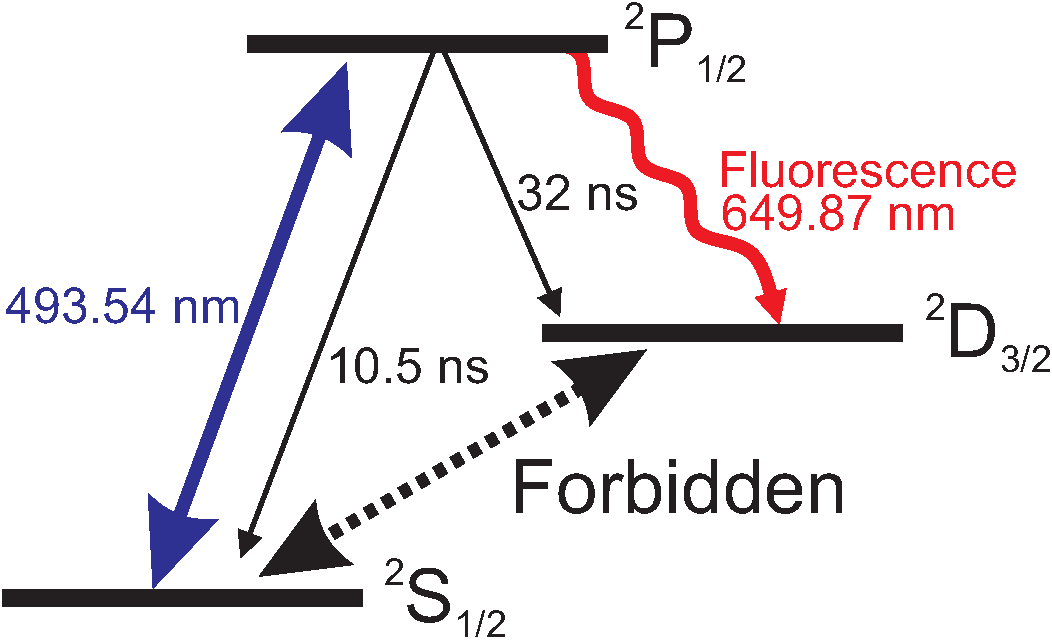
\includegraphics[width=0.5\textwidth]{img/levelscheme.pdf}
\caption{\label{fig.levelscheme} Level scheme for BaTa.} 
\end{figure}
	
%%%%%%

If no discovery is made by the current generation of experiments, the search for \bbonu\ processes will require detectors of larger mass (at least 1 ton), good resolution and extremely low specific background. The \HPXE\ technology has the potential to provide the most sensitive detector in the ton scale, by scaling the detector to a mass in the range of the ton and adding additional handles to further suppress the background. 

One of the most promising possibilities is to develop the technology to unambiguously tag the barium ion produced in the xenon decay, $Xe \rightarrow Ba^{++} + 2 e$. The conceptual idea to tag $Ba^{+}$ is illustrated in Figure \ref{fig.levelscheme2}. A ``blue'' laser of wavelength 493.54 nm excites (``pumps'') the S state, inducing $S \rightarrow P$~transitions, with a lifetime of $\sim$ 10 ns. About 30 \% of the times the \TwoP\ states decay to the state \TwoD, emitting ``red'' (649.86 nm) fluorescence in a characteristic time of 30 ns. The state \TwoD\ is metastable, but a second laser of suitable wavelength (2051.66 nm) can be used to induce the transition to the ground state (this is known as ``deshelving'').  The whole cycle takes less than 50 ns, and therefore several millions of red fluorescence photons can be emitted by a single ion. 

Of course, the practical application of this beautiful conceptual idea is by no means easy, and in fact, it has been shown to be extremely difficult in liquid xenon by the work of the EXO collaboration. However, it may be feasible in an \HPXE\ detector, where a number of fortunate conditions may occur. These conditions are: a) charge reduction of the emitted barium ion, from $Ba^{++}$~to $Ba^{+}$, which can be induced by collisions with xenon atoms, or by the addition of a suitable quencher, such as TEA, as demonstrated by Sinclair et al\footnote{Sinclair.}, b) ``trapping'' of the barium ion ``in situ'' by the surrounding Xe atoms, which result in a very low drift velocity for the ion; c) location of the ion, done by reconstructing the event vertex. 

All the above needs to be demonstrated with a systematic R\&D program, which must also address many other experimental issues such as pressure broadening of the laser, filtering of Rayleigh scattering, etc. Most importantly, such an experimental program must be carried out by an interdisciplinary group, combining the experience in laser spectroscopy and atomic physics, with the experience in \HPXE\ instrumentation.

The on-going collaboration between the IFIC (and other groups of NEXT) and the Center for Pulsed Lasers (CLPU)\footnote{\href{http://www.clpu.es}{http://www.clpu.es}}, a national facility dedicated to ultra-intense lasers research and development has made possible to create precisely the interdisciplinary team needed for a successful R\&D program, which can culminate in a ``Barium-tagging Experiment with a Xenon TPC'' (BEXT). We are currently preparing a white paper which describes the theoretical grounds and details the experimental program to be developed. 

Clearly the construction of a ton-scale \HPXE\ detector implementing a full \BATA\ technology is a very challenging enterprise. On the other hand, we believe that the incremental approach devised by the NEXT collaboration will also work in this case. The construction of the NEW detector is progressing without significant problems thanks to the expertise and know-how gained during DEMO phase, and we expect that NEXT-100 will fully benefit from the experience gained with NEW. Similarly, the \BATA\ technology could be demonstrated in the period of 4 years corresponding to this project,by approaching the problem step by step. 

This is possible only thanks to the collaboration between NEXT and the CLPU.
CLPU is the centre of reference in Spain regarding laser technology, and takes active part in several international and national projects. CLPU enters this co-ordinated project with a full time physicists, who will lead the subproject, Dr. Alicia V. Carpentier who has a well recognised international trajectory in laser-matter interaction. Moreover, CLPU considers this project of high priority and consequently will offer the collaboration of all the scientific department. This consists of a multidisciplinar team with broad experience in laser technology and development, and laser-matter interaction. 

Furthermore, CLPU will support this project with some of the already operating laser systems in its installation. This is extremely important because such systems usually cost of the order of several hundreds of thousand euros which is totally out of the economical scope of this project. The human resources needed to operate the laser systems will be provided by CLPU as well. We will  also like to mention that the small components needed for the construction of the small prototypes will be afforded by the already established NEXT-CLPU collaboration (funds from AdG). In addition, the CLPU and IFIC groups will apply for  \emph{EXPLORA} grants in the next calls.

The different objectives of this subproject are:


\subsection{The \BATA\ program}
The R\&D of the Barium Tagging (\BATA) program includes:

\begin{figure}
\centering
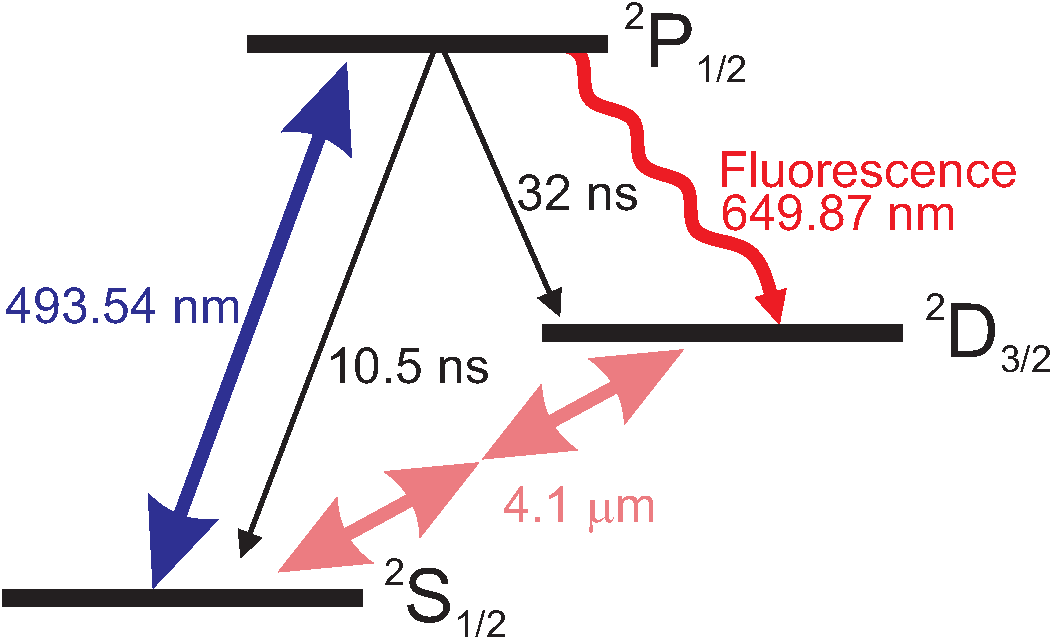
\includegraphics[width=0.5\textwidth]{img/levelscheme2.pdf}
\caption{\label{fig.levelscheme2} Level scheme for BaTa with an infrared deshelving laser.} 
\end{figure}

\begin{itemize}
	\item \textbf{Proof of principle experiment with Ba ions generated by means of an electrical discharge.}
In a first round of experiments we will excite resonantly the S$\leftrightarrow$P transition of Ba$^+$ ions generated by an electrical discharge between two barium electrodes and will collect the fluorescence signal of the P$\rightarrow$D transition (see Figure.\,\ref{fig.levelscheme}). Although this generation method is not ideal because several different species different from Ba ions will be generated, e.g., molecules like BaO or clusters, it does not need a major technological development. It is expected that this initial set of experiments will provide valuable information about the population dynamics in Ba$^+$ ions, and the influence of the different homogenous and in-homogenous broadening mechanisms. It is important to mention that the laser system required for this objective will be provided by the CLPU, and the rest of the material by the ongoing collaboration NEXT-CLPU (e.g., AdG grant).

	\item \textbf{Proof of principle experiment with Ba ions generated by an ion source to be developed.}	
In this objective, in order to get a better approximation of the final conditions of NEXT experiment and with the financial support of a future EXPLORA project, a source of ions will be designed and constructed. This ion source will be based on selective ionisation and mass spectrometry techniques, and it will allow a perfect selection of a target specie. Once the source is ready we will repeat the set of experiments of the previous objective but without any parasitic contribution of unwanted compounds. 
	
	\item \textbf{Proof of principle experiment with Ba ions generated by means of a developed ion source and with a magneto trap.}	
Once the ion source is in operation, in a following objective, we will develop a magneto trap for Ba$^+$  ions. This trap will allow us to have an excellent degree of control over the experimental conditions and to approach the conditions of NEXT. For instance we will carry out different measurements comparing the collected fluorescence signal as a function of the pressure of the Ba$^+$ ions and the pressure of the surrounding environment. These measurements are mandatory because the population dynamics is really sensitive to pressure, i.e., to collisions. 
	
	\item \textbf{Proof of principle experiment with an additional laser for deshelving the D state.}
A possible scenario is that the collisional induced decay between the metastable state D and the ground state S is either not effective or too slow for obtaining an appreciable fluorescence signal. In this situation the population is trapped in the metastable state D  and the fluorescence cycle can not be closed. To avoid this difficulty our approach will be to use a second laser to induce a two photon transition, one photon is forbidden by selection rules, between the states D and S (see Figure.\,\ref{fig.levelscheme2}). This laser must have a wavelength of around 4.1\,$\mu$m which is not easily accesible by commercial laser systems. Our objective is therefore to develop a laser system at this wavelength, and to repeat the experimental matrix defined in previous objectives with two lasers.
	
\end{itemize}

\section{\BATA\ R\&D costs}
\label{bata.costs}

\subsection{R\&D requirements}
The R\&D costs requested to this project are modest. They are:
\begin{enumerate}
\item {\bf A contribution to build an infra-red laser}. The AdG and funds from CLPU cover most of the items needed for the R\&D in 2015 and we fully expect that the EXPLORA project (plus one or more H2020 projects) will cover the R\&D program for the subsequent year. However, a much needed and not fully covered item is a (infra-) red laser of 4.1\,$\mu$m. Such system is needed in our experiments to enhance the transitions between the meta-stable D state in the Ba+ ion and the ground state. On the other hand, it is important to remark that this specific wavelength is not easily accesible by  commercial laser systems, and in fact, there is keen interest in the laser community to develop such laser, due to the fact that this wavelength is not absorbed by the atmosphere and therefore presents many different technological applications. We expect to be able to patent the design and believe it is a clear case of obvious and important industrial return. 
\item {\bf A modest contribution to acquire small equipment and fungible at UPV and US}.
\item {\bf One FPI grant}, to work at the CLPU, in the \BATA\ program. 
\end{enumerate}

\subsection{R\&D costs}
We require a total of 150,000 \euro\ for this program. The bulk of the cost is the development of the infra-red laser (100,000 \euro). To this, we add 25,000 \euro\ for small equipment and fungibles at the US and at the UPV. 

\section{Conclusions}
\label{sec.conclu}

This report summarises the scientific and economic data relevant to the NEXT project, including the R\&D \BATA\ program. The report fully describes the co-funding request to the I+D+i program of ``Challenges of society''. In addition to its scientific excellence, we would like to remark that NEXT is unique in the area of particle physics. As an international collaboration being developed in our national underground laboratory (LSC) and lead by spanish groups, it brings to Spain considerable know-how and external funding. In particular, it is currently the only example of particle-physics experiment in Spain having obtained an advanced grant of the ERC (granted to the spokesperson and PI of this project), 

Of particular interest is also the collaboration with CLPU, which expands the scope of this project to a very interdisciplinar field, including atomic physics and laser-matter interaction. The prospects of industrial returns in the \BATA\ program appear very high, in particular thanks to the development of infra-red laser technology and controlled ions sources, areas with an increasing number of industrial and scientific applications. 

Last but not least, the NEXT experiment, and/or the future BEXT experiment, including the \BATA\ technology have the clear potential of leading a major scientific discovery.

\end{document}

